%!TeX spellcheck = en
% Final presentation, built on the course TUKL Beamer template.
% Content source: reports/final_report/main.tex (final project report).
% Build: tectonic slides.tex
\documentclass{beamer}
\usetheme[noptsans,navigation=true , FB=Informatik, frametotal=false]{TUKL}
\setbeamertemplate{navigation symbols}{}
\usepackage{xcolor}
\usepackage[english]{babel}
\usepackage[ddmmyyyy]{datetime}
\usepackage{hyperref}
\usepackage{amssymb}
\usepackage{tikz}
\usetikzlibrary{arrows.meta, positioning}
\usepackage{pgfplots}
\pgfplotsset{compat=1.18}

% ===============================================
% TODO: set to the actual presentation date
\newcommand{\presentationDate}{30.09.2026}
% ===============================================

\title{\vspace{0.5em}Machine Learning and Deep Learning}
\author{Purna Chandra Nandigana}
\date[\presentationDate]{
\includegraphics[width=0.5\textwidth]{logos/group-logo-text-new.png} \hspace{5em} \presentationDate}

% Flow-diagram style used on several slides (same look as the reference deck)
\tikzset{
  flowbox/.style={rectangle, rounded corners, draw=black, align=center, inner sep=3pt},
  flowarr/.style={-{To[length=1.6mm]}},
}
\newcommand{\takeaway}[1]{\par\vspace{0.4em}\noindent\textbf{Key Takeaway:} #1}

\begin{document}

\maketitle

% ===================== 2 =====================
\begin{frame}{What problem am I solving?}
\begin{itemize}
  \item \textbf{Problem:} flag every anomalous timestep in 18-sensor recordings of a batch-distillation plant (1\,Hz).
  \item \textbf{Challenge:} the 28 training runs have \emph{no labels}.
  \begin{itemize}
    \item 10 validation runs are labelled (24\% anomalous)
    \item 53 test runs are scored on the Codabench portal (binary F1)
  \end{itemize}
  \item \textbf{Approach:} learn what \emph{normal} looks like, then flag departures from it (novelty detection).
\end{itemize}
\takeaway{No anomaly labels for training, so the model must learn normal behaviour.}
\end{frame}

% ===================== 3 =====================
\begin{frame}{What does the data look like?}
\begin{center}
\small
\begin{tabular}{|l|c|c|l|}
\hline
\textbf{Split} & \textbf{Runs} & \textbf{Timesteps} & \textbf{Labels} \\
\hline
Train & 28 & 189{,}444 & none \\
Validation & 10 & 79{,}688 & per timestep \\
Test & 53 & 316{,}024 & hidden (portal) \\
\hline
\end{tabular}
\end{center}
\begin{itemize}
  \item \textbf{Sensors:} temperatures, flows, pressures and levels
  \item \textbf{Anomaly rate per validation run:} from 0.8\% to 81\%
  \item \textbf{No separate test labels:} the 10 labelled runs are used for tuning \emph{and} for every local metric
\end{itemize}
\takeaway{Very few labelled runs, and they differ a lot from each other.}
\end{frame}

% ===================== 4 =====================
\begin{frame}{Phase 1: Where did I start?}
\begin{columns}[T]
\column{0.55\textwidth}
\begin{itemize}
  \item \textbf{Baseline:} Isolation Forest on 216 tabular features\\ $\rightarrow$ val.\ F1 = 0.437
  \item \textbf{First deep model:} hybrid of a shallow CNN autoencoder and a window Isolation Forest (weights 0.85 / 0.15)
  \item Its reported F1 $\approx$ 0.62 was measured on \emph{window-level} labels and could not be reproduced
\end{itemize}
\column{0.42\textwidth}
\centering
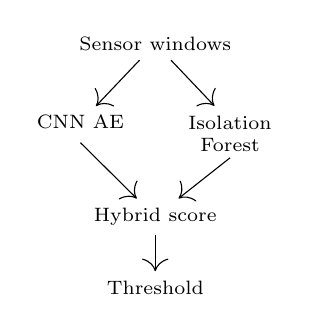
\begin{tikzpicture}[font=\scriptsize]
\node (w) at (0,0) {Sensor windows};
\node (c) at (-0.95,-1.0) {CNN AE};
\node (i) at (0.95,-1.0) {Isolation};
\node at (0.95,-1.28) {Forest};
\node (h) at (0,-2.2) {Hybrid score};
\node (t) at (0,-3.1) {Threshold};
\draw[flowarr] (w) -- (c); \draw[flowarr] (w) -- (i);
\draw[flowarr] (c.south) ++(0,-0.05) -- (h); \draw[flowarr] (0.95,-1.45) -- (h);
\draw[flowarr] (h) -- (t);
\end{tikzpicture}
\end{columns}
\vspace{0.3em}
\takeaway{The starting point was a hybrid model whose numbers could not yet be trusted.}
\end{frame}

% ===================== 5 =====================
\begin{frame}{Phase 1: What did I have to fix first?}
\begin{itemize}
  \item \textbf{Six correctness bugs} found while rebuilding the notebooks into one pipeline:
  \begin{itemize}
    \item windows crossed run boundaries
    \item threshold taken off by one
    \item Isolation Forest features flattened wrongly
    \item scoring per window instead of per timestep
    \item training reverted from 50 to 10 epochs
    \item fusion weight hand-set instead of tuned
  \end{itemize}
  \item \textbf{Result after fixing:} hybrid val.\ F1 = 0.494
  \item \textbf{Portal:} 0.399 (public) / 0.471 (private)
\end{itemize}
\takeaway{Correct evaluation first; only then do the numbers mean anything.}
\end{frame}

% ===================== 6 =====================
\begin{frame}{Phase 1: How did the autoencoder improve?}
\begin{center}
\small
\begin{tabular}{|l|c|c|}
\hline
\textbf{Round} & \textbf{CNN F1} & \textbf{CNN ROC-AUC} \\
\hline
1: corrected pipeline & 0.408 & 0.574 \\
2: checkpoint selection & 0.458 & 0.614 \\
3: dilated architecture & 0.484 & 0.605 \\
\hline
\end{tabular}
\end{center}
\begin{itemize}
  \item \textbf{Checkpoint selection:} keep the best validation epoch, not the last
  \item \textbf{Dilated architecture:} wider view of time (61 timesteps)
  \item \textbf{Problem left:} ROC-AUC stayed near 0.6 and the threshold flagged up to 89\% of timesteps
\end{itemize}
\takeaway{F1 went up, but ranking quality did not: the score itself was the bottleneck.}
\end{frame}

% ===================== 7 =====================
\begin{frame}{Phase 2: How does the final pipeline work?}
\begin{center}
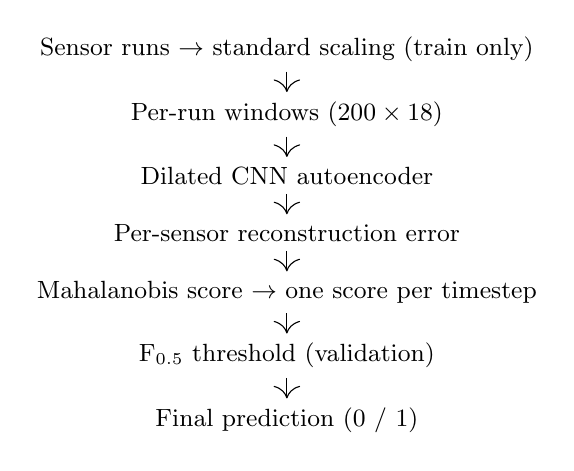
\begin{tikzpicture}[node distance=0.26cm, font=\small]
\node (a) {Sensor runs $\rightarrow$ standard scaling (train only)};
\node[below=of a] (b) {Per-run windows ($200 \times 18$)};
\node[below=of b] (c) {Dilated CNN autoencoder};
\node[below=of c] (d) {Per-sensor reconstruction error};
\node[below=of d] (e) {Mahalanobis score $\rightarrow$ one score per timestep};
\node[below=of e] (f) {F$_{0.5}$ threshold (validation)};
\node[below=of f] (g) {Final prediction (0 / 1)};
\foreach \x/\y in {a/b,b/c,c/d,d/e,e/f,f/g} \draw[flowarr] (\x) -- (\y);
\end{tikzpicture}
\end{center}
\takeaway{Same autoencoder as Phase 1, but a new score and a new threshold.}
\end{frame}

% ===================== 8 =====================
\begin{frame}{Phase 2: How does the CNN autoencoder learn normal behaviour?}
\begin{columns}[T]
\column{0.56\textwidth}
\begin{itemize}
  \item \textbf{Input:} window of 200 timesteps $\times$ 18 sensors
  \item \textbf{Encoder:} 4 dilated residual blocks (dilation 1, 2, 4, 8) $\rightarrow$ MaxPool
  \item \textbf{Decoder:} ConvTranspose1d $\rightarrow$ 2 residual blocks $\rightarrow$ Conv1d
  \item \textbf{Training:} MSE, Adam (lr $10^{-3}$), batch 64, 50 epochs, best checkpoint every 5 epochs
\end{itemize}
\column{0.40\textwidth}
\centering
\textbf{Model Flow}
\begin{itemize}
  \item Input $18\times200$
  \item Dilated blocks (32, 32, 32, 64)
  \item MaxPool $\rightarrow 64\times100$
  \item ConvTranspose1d
  \item Dilated blocks (32, 32)
  \item Output $18\times200$
\end{itemize}
\end{columns}
\vspace{0.3em}
\takeaway{59,858 parameters; the bottleneck makes it good only at normal data.}
\end{frame}

% ===================== 9 =====================
\begin{frame}{Phase 2: How is the anomaly score calculated?}
\begin{itemize}
  \item \textbf{Before:} one flat error averaged over all sensors, so a spike on one precise sensor was diluted
  \item \textbf{Now:} one error per sensor, $e_w \in \mathbb{R}^{18}$
\end{itemize}
\begin{block}{Per-Sensor Mahalanobis Score}
\[
s(w) = (e_w - \mu)^{\top}\, \Sigma^{-1}\, (e_w - \mu)
\]
\end{block}
\begin{itemize}
  \item \textbf{$\mu, \Sigma$:} fitted on normal validation windows (Ledoit--Wolf)
  \item \textbf{Per timestep:} mean score of all windows that contain it
\end{itemize}
\takeaway{Each sensor is judged against its own normal error level.}
\end{frame}

% ===================== 10 =====================
\begin{frame}{Phase 2: How is the decision boundary selected?}
\begin{center}
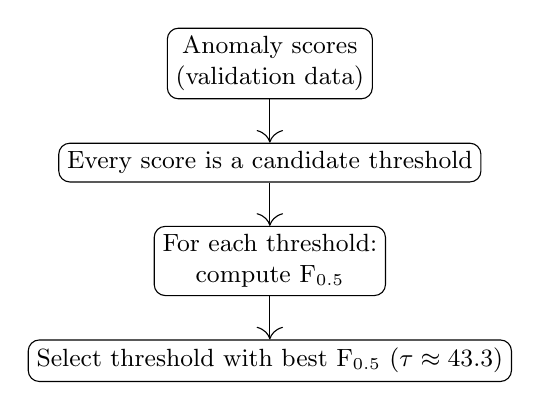
\begin{tikzpicture}[node distance=0.55cm, font=\small]
\node[flowbox] (a) {Anomaly scores\\(validation data)};
\node[flowbox, below=of a] (b) {Every score is a candidate threshold};
\node[flowbox, below=of b] (c) {For each threshold:\\compute F$_{0.5}$};
\node[flowbox, below=of c] (d) {Select threshold with best F$_{0.5}$ ($\tau \approx 43.3$)};
\draw[flowarr] (a) -- (b); \draw[flowarr] (b) -- (c); \draw[flowarr] (c) -- (d);
\end{tikzpicture}
\end{center}
\textbf{Key Idea:} F$_{0.5}$ weights precision above recall, which stops the model from flagging most of the data.
\end{frame}

% ===================== 11 =====================
\begin{frame}{Phase 2: Did the new score help?}
\begin{center}
\small
\begin{tabular}{|l|c|c|}
\hline
\textbf{Metric (validation)} & \textbf{Round 3} & \textbf{Round 4} \\
\hline
F1 & 0.484 & \textbf{0.581} \\
Precision / recall & 0.347 / 0.796 & 0.601 / 0.562 \\
ROC-AUC & 0.605 & \textbf{0.768} \\
Flagged (true 0.24) & 0.894 & 0.224 \\
\hline
\end{tabular}
\end{center}
\begin{itemize}
  \item \textbf{ROC-AUC $+0.16$:} better ranking, independent of the threshold
  \item \textbf{Portal:} 0.471 $\rightarrow$ \textbf{0.59}
\end{itemize}
\takeaway{Changing the score, not the network, gave the largest gain of the project.}
\end{frame}

% ===================== 12 =====================
\begin{frame}{Phase 2: Did fusion with LOF help?}
\begin{itemize}
  \item \textbf{Test:} fuse CNN with a Local Outlier Factor detector (contributed by my teammate)
  \item \textbf{Weight} chosen by 5-fold cross-validation grouped by run
\end{itemize}
\begin{center}
\small
\begin{tabular}{|l|c|c|c|}
\hline
\textbf{Val.\ F1} & \textbf{CNN only} & \textbf{LOF only} & \textbf{Hybrid} \\
\hline
raw features & \textbf{0.592} & 0.461 & 0.549 \\
standardised & \textbf{0.568} & 0.481 & 0.568 \\
\hline
\end{tabular}
\end{center}
\begin{itemize}
  \item 9 of 10 folds chose the CNN alone (LOF weight 0.03 / 0.00)
\end{itemize}
\takeaway{Fusion was rejected; the final model is the CNN autoencoder alone.}
\end{frame}

% ===================== 13 =====================
\begin{frame}{Final Performance Comparison (Test Set)}
\begin{center}
\begin{tabular}{|c|c|c|}
\hline
\textbf{Model} & \textbf{Val.\ F1} & \textbf{Portal F1 (Test)} \\
\hline
Phase 1: hybrid & 0.494 & 0.399 / 0.471 \\
Phase 2: Mahalanobis score & 0.581 & 0.59 \\
Phase 2: CNN only (final) & 0.602 & \textbf{0.63} \\
\hline
\end{tabular}
\end{center}
\begin{itemize}
  \item Final model: val.\ ROC-AUC 0.763
  \item 0.59 $\rightarrow$ 0.63: a new training run of the same method (run-to-run spread about $\pm0.02$)
\end{itemize}
\textbf{Key Insight:} The CNN autoencoder with Mahalanobis scoring achieves the best result, portal F1 = 0.63.
\end{frame}

% ===================== 14 =====================
\begin{frame}{How did performance change across the phases?}
\begin{center}
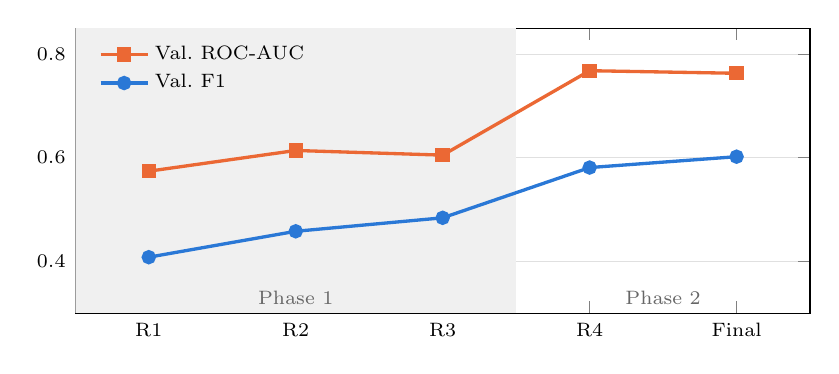
\begin{tikzpicture}
\begin{axis}[
  width=0.9\textwidth, height=5.2cm,
  ymin=0.3, ymax=0.85, xmin=0.5, xmax=5.5,
  xtick={1,2,3,4,5}, xticklabels={R1,R2,R3,R4,Final},
  tick label style={font=\scriptsize}, ymajorgrids, grid style={black!12},
  legend style={font=\scriptsize, draw=none, fill=none, at={(0.02,0.98)}, anchor=north west},
  legend cell align=left]
  \fill[black!6] (axis cs:0.5,0.3) rectangle (axis cs:3.5,0.85);
  \node[font=\scriptsize, text=black!60] at (axis cs:2,0.33) {Phase 1};
  \node[font=\scriptsize, text=black!60] at (axis cs:4.5,0.33) {Phase 2};
  \addplot[color={rgb,255:red,235;green,104;blue,52}, line width=1.2pt, mark=square*] coordinates {(1,0.574) (2,0.614) (3,0.605) (4,0.768) (5,0.763)};
  \addlegendentry{Val.\ ROC-AUC}
  \addplot[color={rgb,255:red,42;green,120;blue,214}, line width=1.2pt, mark=*] coordinates {(1,0.408) (2,0.458) (3,0.484) (4,0.581) (5,0.602)};
  \addlegendentry{Val.\ F1}
\end{axis}
\end{tikzpicture}
\end{center}
\takeaway{Phase 1 raised F1 slowly; Phase 2 moved the ranking quality itself.}
\end{frame}

% ===================== 15 =====================
\begin{frame}{How reliable is the final result?}
\begin{itemize}
  \item \textbf{Tested after the final submission} (none adopted):
  \begin{itemize}
    \item F1-optimal threshold: +0.024 val.\ F1, but flags 84\% of test
    \item Per-run normalisation: ROC-AUC 0.769 $\rightarrow$ 0.677
    \item Normal model fitted on train: ROC-AUC 0.611
  \end{itemize}
  \item \textbf{Leave-one-run-out:} validation is optimistic by 0.070 ROC-AUC and 0.058 F1
  \item \textbf{Val.\ vs test:} 24\% vs 62\% of timesteps flagged at the same threshold
\end{itemize}
\takeaway{The method held up, but validation numbers should be read as optimistic.}
\end{frame}

% ===================== 16 =====================
\begin{frame}{What are the key parameters of the final system?}
\begin{center}
\small
\begin{tabular}{|l|l|}
\hline
\textbf{Component} & \textbf{Parameter Value} \\
\hline
Windowing & Window size = 200, train stride = 10 \\
CNN Autoencoder & Dilations = 1, 2, 4, 8 \\
CNN Autoencoder & Filters = 32, 32, 32, 64 \\
CNN Autoencoder & Batch size = 64 \\
CNN Autoencoder & Learning rate = 1e-3, 50 epochs \\
Scoring & Mahalanobis, Ledoit--Wolf covariance \\
Threshold & F$_{0.5}$, $\tau \approx 43.3$ \\
\hline
\end{tabular}
\end{center}
\textbf{Key Insight:} Performance depended most on how the error is scored and thresholded.
\end{frame}

% ===================== 17 =====================
\begin{frame}{Summary \& Next Steps}
\begin{itemize}
  \item \textbf{Summary:} dilated CNN autoencoder with per-sensor Mahalanobis scoring and an F$_{0.5}$ threshold.
  \item \textbf{Result:} portal F1 = \textbf{0.63} (val.\ F1 0.602, ROC-AUC 0.763).
  \item \textbf{Key Outcome:} Phase 2's new score lifted ROC-AUC from 0.605 to 0.768.
  \item \textbf{Next Steps:}
  \begin{itemize}
    \item Leave-one-run-out validation for every tuning step
    \item Confirm how the portal computes F1
    \item Average over several training seeds
  \end{itemize}
\end{itemize}
\textbf{Final Message:} How the model's error is scored mattered more than model size.
\end{frame}

\end{document}
